\documentclass{ctexart}%若为article则section左靠齐
\usepackage{ctex}
%纸张设计
\usepackage[a4paper,left=25mm,right=25mm,bottom=25mm,top=30mm]{geometry}

%目录的设计
\usepackage{titletoc}
\usepackage{titlesec}

%字体设计
%\usepackage{fontspec}
\newcommand{\chuhao}{\fontsize{42pt}{\baselineskip}\selectfont}     %初号  
\newcommand{\xiaochuhao}{\fontsize{36pt}{\baselineskip}\selectfont} %小初号  
\newcommand{\yihao}{\fontsize{28pt}{\baselineskip}\selectfont}      %一号  
\newcommand{\erhao}{\fontsize{21pt}{\baselineskip}\selectfont}      %二号  
\newcommand{\xiaoerhao}{\fontsize{18pt}{\baselineskip}\selectfont}  %小二号  
\newcommand{\sanhao}{\fontsize{15.75pt}{\baselineskip}\selectfont}  %三号  
\newcommand{\sihao}{\fontsize{14pt}{\baselineskip}\selectfont}       %四号  
\newcommand{\xiaosihao}{\fontsize{12pt}{\baselineskip}\selectfont}  %小四号  
\newcommand{\wuhao}{\fontsize{10.5pt}{\baselineskip}\selectfont}    %五号  
\newcommand{\xiaowuhao}{\fontsize{9pt}{\baselineskip}\selectfont}   %小五号  
\newcommand{\liuhao}{\fontsize{7.875pt}{\baselineskip}\selectfont}  %六号  
\newcommand{\qihao}{\fontsize{5.25pt}{\baselineskip}\selectfont}    %七号

%标题设计
\titleformat*{\section}{\centering\xiaoerhao\bfseries}
\titleformat*{\subsection}{\sihao\bfseries}
\titleformat*{\subsubsection}{\xiaosihao\bfseries}

%行距设计
\usepackage{setspace}
\renewcommand{\baselinestretch}{1.25}
\usepackage{array}%图表行距

%标题设计
\title{这里是标题}
\author{Qtvz}
\date{}%去除时间

%页眉设计
\usepackage{fancyhdr}
\pagestyle{fancy}
\lhead{}
\rhead{}
\chead{Qtvz's bachelorthesis}

%双文摘要控制
\usepackage{chngpage}

%参考文献上标
\newcommand{\upcite}[1]{\textsuperscript{\textsuperscript{\cite{#1}}}}

%图片包
\usepackage{graphicx}
\usepackage{subfigure}
\usepackage{wrapfig}%混排

%添加超链接,并去除边框
\usepackage[colorlinks,linkcolor=black,anchorcolor=black,citecolor=black,urlcolor=black]{hyperref}

%图表包
\usepackage{xcolor}%定义了一些颜色
\usepackage{colortbl,booktabs}%第二个包定义了几个*rule
\usepackage{tabu}

%控制图片、表格caption
\usepackage{caption}
\captionsetup[table]{
	%labelsep=newline,%换行
	%singlelinecheck=false,%居左
	font=large,
	labelfont=bf,
	textfont=bf,
	labelsep=quad%去除冒号
}

\captionsetup[figure]{
	font=large,
	labelfont=bf,
	textfont=bf,
	labelsep=quad
}

%图片caption章节编号
\renewcommand {\thetable} {\thesection{}.\arabic{table}} 
\renewcommand {\thefigure} {\thesection{}.\arabic{figure}}
\renewcommand{\thesubfigure}{\large(\alph{subfigure})}
\newcommand{\fref}[1]{\thesection.\ref{#1}}

%公式包
\usepackage{amsmath}
\usepackage{cases}
\usepackage{siunitx}%角度符号

%文字边框
\usepackage{framed}

%代码边框
\usepackage{listings}

%插入PDF页
\usepackage{pdfpages}

%开始文档
\begin{document}
	%显示标题
	\maketitle
	\thispagestyle{plain}
	\setcounter{page}{1}%页码重置
	\pagenumbering{roman}
	\thispagestyle{plain}
	%摘要
	\begin{center}	
		\LARGE{\textbf{摘要}}	
	\end{center}
	\begin{adjustwidth}{1cm}{1cm}
		\large
		\hspace{2em}这里是中文摘要
		\newline
		\textbf{关键词:}这里是关键词
	\end{adjustwidth}
	\newpage
	\thispagestyle{plain}
	\begin{center}	
		\LARGE{\textbf{Abstract}}	
	\end{center}
	\begin{adjustwidth}{1cm}{1cm}
		\large
		\hspace{1.8em}Here we go the abstract.
		\newline
		\textbf{Keywords:}Your keyword.
	\end{adjustwidth}
	\thispagestyle{plain}
	%目录
	\newpage
	%生成目录
	\tableofcontents
	%一级标题目录连接线
	\titlecontents{section}
	[0mm]
	{\bf \large}%
	{\contentslabel{2.5em}}%
	{}%
	{\titlerule*[0.5pc]{$\cdot$}\contentspage\hspace*{-0.3mm}}%
	%页脚设计
	\thispagestyle{fancy}
	%正文
	\newpage
	\thispagestyle{fancy}
	\setcounter{page}{1}
	\pagenumbering{arabic}
	%section取消编号并呈现在目录中
	\section*{第一章\quad aa}
	\addcontentsline{toc}{section}{第一章\quad aa}
	\setcounter{section}{1}
	\setcounter{figure}{1}
	\setcounter{table}{1}
	\subsection{11}
	\subsubsection{111}
	\xiaosihao
	112121\upcite{Qtvz's,11,la}\par
	\subsubsection{112}
	\subsection{113}
	\newpage
	\section*{第二章\quad bb}
	\addcontentsline{toc}{section}{第二章\quad bb}
	\setcounter{section}{2}
	\setcounter{subsection}{0}
	\setcounter{figure}{1}
	\setcounter{table}{1}
	\subsection{21}
	\subsubsection{211}
	\sihao
	Such as fig\fref{Wullf}\par 
	\begin{figure}[htpb]
		\setcounter{figure}{0}
		\subfigure[\normalsize fig1]{
			\begin{minipage}[t]{0.25\linewidth}
				\centering
				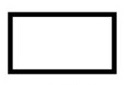
\includegraphics[width=1.2in]{figs/lapic/fig1}
				\label{Wullf}
			\end{minipage}%
		}%
		\subfigure[\normalsize fig2]{
			\begin{minipage}[t]{0.25\linewidth}
				\centering
				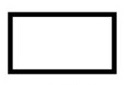
\includegraphics[width=1.2in]{figs/lapic/fig1}
				\label{Schmidt}
			\end{minipage}%
		}%	
		%这个回车键很重要 \quad也可以,回车则为2X2,否则为一行
		\subfigure[\normalsize fig3]{
			\begin{minipage}[t]{0.25\linewidth}
				\centering
				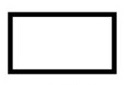
\includegraphics[width=1.2in]{figs/lapic/fig1}
				\label{adarc}
			\end{minipage}
		}%
		\subfigure[\normalsize fig4]{
			\begin{minipage}[t]{0.25\linewidth}
				\centering
				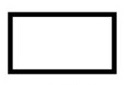
\includegraphics[width=1.2in]{figs/lapic/fig1}
				\label{adarea}
			\end{minipage}
		}%
		\caption{figs}
		\label{ste}
	\end{figure}
	\subsubsection{212}
	22\ref{frou}:\par
	\setcounter{equation}{0}
	\begin{equation}\label{frou}
		f(\rho,\theta)=
		\left\{ 
		\begin{array}{c}
		\rho^2=x^2+y^2 \\ 
		x=\rho\cos\theta \\ 
		y=\rho\sin\theta
		\end{array}
		\right.
	\end{equation}\par
	\textbf{\bfseries 在同一个平面内,三个不在同一条直线上的点确定唯一一个圆。}
	\ang{0}为W-E
		\begin{equation}\label{getqj}
			OC=\rho\tan(\frac{\pi}{4}-\frac{\beta}{2})
		\end{equation}\par
	\subsection{22}
	\subsubsection{221}
	\begin{framed}
		$import\quad numpy\quad as\quad np$
	\end{framed}
	\subsubsection{222}
	\clearpage%遇到由于图片无法换页可尝试
	\section*{第三章\quad cc}
	\addcontentsline{toc}{section}{第三章\quad cc}
	\setcounter{section}{3}
	\setcounter{subsection}{0}	
	\setcounter{figure}{1}
	\setcounter{table}{0}
	\subsection{31}
	\begin{center}
		\large \textbf{代码3.1\quad 单张图片的插入并编排}
	\end{center}
	\begin{lstlisting}[language={[ANSI]C},keywordstyle=\color{blue!70},commentstyle=\color{red!50!green!50!blue!50},frame=shadowbox,rulesepcolor=\color{red!20!green!20!blue!20}] 
	    \usepackage{graphicx}
	    \begin{document}
	    \end{document}	
	\end{lstlisting}\par 
	\subsection{32}
	如表\ref{picsea}所示\par 
	aa
	\begin{framed}
	$\backslash begin\{wrapfigure\}\{linenum\}[seat][Exceeding\quad length]$\par
	$\qquad\qquad\qquad\quad\quad\quad\{width\}\langle{fig}\rangle\backslash end\{wrapfigure\}$
	\end{framed}
	\begin{table}[h]
		\xiaosihao
		\centering
		\caption{图文混排seat参数}
		\label{picsea}
		\renewcommand\arraystretch{1.5}
		\begin{tabular}{p{1cm}p{1.5cm}p{5.6cm}p{3.6cm}}
			\hline
			编号 & 参数 & 效果 & 备注 \\
			\hline
			a & r,R & 图形位于文本的右边 & 浮动控制\\
			b & l,L & 图形位于文本的左边 & 浮动控制\\
			c & i,R & 图形位于页面靠里的一边 & 仅用于双面格式中\\
			d & o,O & 表示图形位于页面靠外的一边 & 双面格式\\
			\hline
		\end{tabular}
	\end{table}
	\clearpage
	\section*{第四章\quad dd}
	\addcontentsline{toc}{section}{第四章\quad dd}
	\setcounter{section}{4}
	\setcounter{subsection}{0}
	\setcounter{figure}{1}
	\setcounter{table}{0}
	\subsection{41}
	\subsubsection{411}
	\subsubsection{412}
	\subsection{42}
	\subsubsection{421}
	\subsubsection{422}
	\subsubsection{423}
	\begin{table}[h]
		\xiaosihao
		\centering
		\caption{thispagestyle各参数效果}
		\label{ttps}
		\renewcommand\arraystretch{1.5}
		\begin{tabular}{p{1cm}p{2.5cm}p{5cm}p{4.7cm}}
			\hline
			编号 & 参数 & 效果 & 备注 \\
			\hline
			a & plain & 仅显示页码 & 无页眉\\
			b & empty & 不显示所有页眉与页脚 & 常应用于扉页\\
			c & headings & 页眉处显示当前标题 & 与当前内容有关,无页脚\\
			d & myheadings & 页眉页码为自定义信息 & 作者自定义\\
			\hline
		\end{tabular}
	\end{table}\par 
	\newpage
	\addcontentsline{toc}{section}{参考文献}
	\newpage
	\wuhao
	\bibliographystyle{gbt7714-2005}%引用顺序排序
	\bibliography{ref}
	\newpage
	\addcontentsline{toc}{section}{附录}
	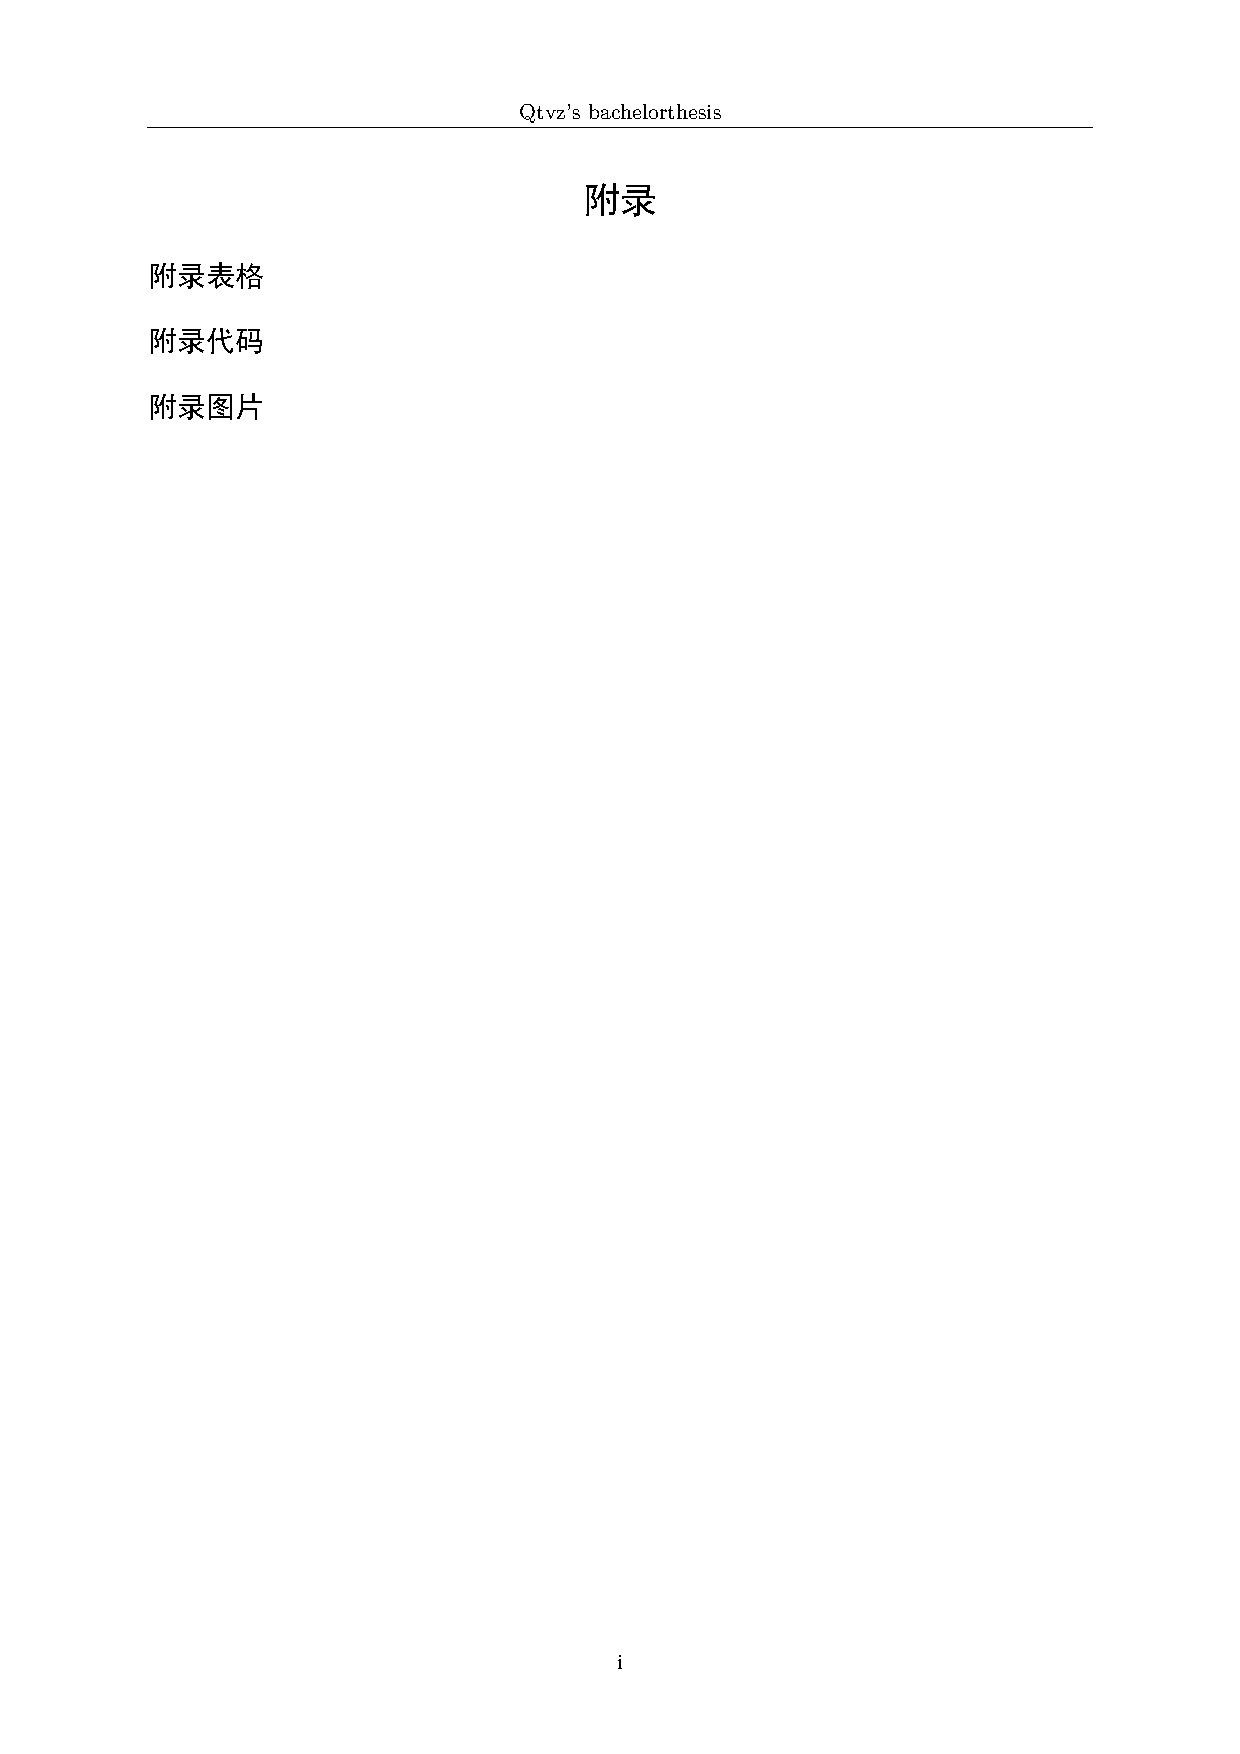
\includepdf[pages=1]{others/par.pdf}
\end{document}